\documentclass[nobib]{tufte-handout}
% \documentclass[fleqn,reqno,12pt]{article}

%========================================
% Packages
%========================================

\usepackage[nographicx, nohyperref, nosubcaption, nogb4e]{mfpackages}
\usepackage{mfenvironments}
\usepackage{mfcommands}
% for info boxes
\usepackage{newfloat, caption}
\DeclareCaptionType{InfoBox}


%========================================
% Bibliography
%========================================

\bibliography{references.bib}

%========================================
% General Layout Tweaks
%========================================

% \usepackage[margin=2cm]{geometry}

% Itemize
\renewcommand{\labelitemi}{\large{$\mathbf{\cdot}$}}    % itemize symbols
\renewcommand{\labelitemii}{\large{$\mathbf{\cdot}$}}
\renewcommand{\labelitemiii}{\large{$\mathbf{\cdot}$}}
\renewcommand{\labelitemiv}{\large{$\mathbf{\cdot}$}}
% Description
\renewcommand{\descriptionlabel}[1]{\hspace\labelsep\textsc{#1}}

% Figure Captions
\usepackage{caption} % use corresponding myfiguresize!
\setlength{\captionmargin}{20pt}
\renewcommand{\captionfont}{\small}
\setlength{\belowcaptionskip}{7pt} % standard is 0pt

%========================================
% Define colors and comment functions
%========================================

\usepackage{xcolor}
\definecolor{firebrick}{RGB}{178,34,34}
\definecolor{DarkGreen}{RGB}{34,178,34} 
\definecolor{DarkOrange}{RGB}{255,100,50}
\renewcommand{\mf}[1]{\textcolor{firebrick}{[mf: #1]}}  
\newcommand{\tr}[1]{\textcolor{DarkOrange}{[tr: #1]}}  
%========================================
% Configuring the R code presentation
%========================================

\usepackage{courier}
\usepackage{listings}
\usepackage{color}
% the following defines the layout for the R code
\lstset{ %
  language=R,                     % the language of the code
  basicstyle=\footnotesize\ttfamily, % size and type of the fonts that are used for the code
  numbers=left,                   % where to put the line-numbers
  numberstyle=\tiny\color{gray},  % the style that is used for the line-numbers
  stepnumber=1,                   % the step between two line-numbers. If it's 1, each line
                                  % will be numbered
  numbersep=5pt,                  % how far the line-numbers are from the code
  backgroundcolor=\color{white},  % choose the background color. You must add \usepackage{color}
  showspaces=false,               % show spaces adding particular underscores
  showstringspaces=false,         % underline spaces within strings
  showtabs=false,                 % show tabs within strings adding particular underscores
  frame=single,                   % adds a frame around the code
  rulecolor=\color{black},        % if not set, the frame-color may be changed on line-breaks within not-black text (e.g. commens (green here))
  tabsize=2,                      % sets default tabsize to 2 spaces
  captionpos=b,                   % sets the caption-position to bottom
  breaklines=true,                % sets automatic line breaking
  breakatwhitespace=false,        % sets if automatic breaks should only happen at whitespace
  title=\lstname,                 % show the filename of files included with \lstinputlisting;
                                  % also try caption instead of title
  keywordstyle=\color{blue},      % keyword style
  commentstyle=\color{DarkGreen}, % comment style
  stringstyle=\color{DarkOrange}, % string literal style
  escapeinside={\%*}{*)},         % if you want to add a comment within your code
  morekeywords={*, ...}            % if you want to add more keywords to the set
}

% this is for showing the R output
\lstnewenvironment{rc}[1][]{\lstset{language=R}}{}

% this is for inline R code
\newcommand{\ri}[1]{\lstinline{#1}}  %% Short for 'R inline'

%========================================
% Article Header 
%========================================


\title{Hands-on non-technical tutorial for Bayesian mixed effects regression}
\author{Michael Franke \& Timo Roettger}
\date{}

%========================================
% Article Body
%========================================

\begin{document}
\maketitle

\begin{abstract}
  \noindent Generalized linear models with mixed effects are very versatile and handy tools for statistical inference. Bayesian approaches to applying these models have also recently become more popular. This tutorial provides an accessible, non-technical introduction to the use and feel of Bayesian mixed effects regression models. The focus is on data from a factorial-design experiment. \\
  
  \medskip
  
  \noindent \textbf{This tutorial should take you about 1 hour.}
\end{abstract}

\section{Motivation \& intended audience}

This tutorial provides a very basic introduction to Bayesian regression modeling using R \citep{Manual}. We wrote this tutorial with a particular reader in mind. If you have used R before and if you have a basic understanding of linear regression and now you want to find out what a Bayesian approach has to offer, this tutorial is for you. In comparison to other introductions \citep[e.g.][]{SorensenHohensteinb2016:Bayesian-linear}, this tutorial remains very conceptual. We don’t want to ``sell Bayes'' to you, and we do not want to scare you away with mathematical details. We just want to give you an impression of how a Bayesian regression analysis looks and feels. So no reason to be afraid! But also: no reason to be bored, because we \emph{will} cover all the essential concepts and we \emph{will} explain how to run and interpret the output of a Bayesian regression analysis using the wonderful R package \texttt{brms} written by Paul \citep{buerkner2016brms}.

If you don’t have any experience with regression modeling, you will probably still be able to follow but you might also easily catch up by doing a crash course. To bring you up to speed, we recommend the excellent two-part tutorial by Bodo \citep{Winter2013:Linear-models-a} on mixed effects regression in a non-Bayesian ---a.k.a.~classical or frequentist--- paradigm. In a sense, this tutorial could be considered part three of Bodo's nice and lofty introduction. We will, for example use the same data set.


\section{The data}
\label{sec:data}

Now, what do we as experimental researchers often do? We often have a research hypothesis about how aspects of nature relate to each other. For example, we might want to know whether voice pitch differs across female and male speakers, and whether it differs across social contexts (say: informal or polite contexts). --- To answer our questions, we lure a group of people into the lab, we ask them to say different words in different social contexts, we record their voices, and record some numbers, e.g., the pitch values.

\citet{Winter2013:Linear-models-a} looks at data of this sort \citep[taken from][]{WinterGrawunder2012:The-Phonetic-Pr} and so will we. The data is obtainable from \dots \mf{how to get the data}. To load the data into R, copy the file \texttt{FILENAME} \dots \mf{describe set up} and type this into an R console (perhaps using
RStudio \mf{insert URL})\footnote{If you are familiar with the previous tutorials by \citet{Winter2013:Linear-models-a}, it might help you to know that we have (courteously) massaged the data a tiny little bit: we have already removed one line with missing data and we have changed the way the variable
\texttt{scenario} is represented, so that it gets treated (correctly) later on in the regression analysis without much further ado.}

\medskip

\begin{lstlisting}[language=R]
  # load the data into variable 'politedata'
  politedata = read.csv(file = 'MyData.csv')     
\end{lstlisting}

\vspace*{-0.5cm}

\noindent If we now type \ri{head(politedata)}, we see the first six lines of the data, like so:

\medskip


\begin{rc}
> head(politedata)
  subject gender scenario attitude  freq
1      F1      F       S1      pol 213.3
2      F1      F       S1      inf 204.5
3      F1      F       S2      pol 285.1
4      F1      F       S2      inf 259.7
5      F1      F       S3      pol 203.9
6      F1      F       S3      inf 286.9
\end{rc}

\medskip

\noindent What is important for us here is that there are multiple measurements for the same subjects. We have a measurement of pitch frequency \mf{is that the right term?} for different subjects, who are (crudely) classified as either male or female, and different scenarios (e.g., words/sentences to pronounce). The experiment has manipulated whether the scenario took place in a polite or informal context. This is indicated by the variable \texttt{attitude}.

What aspects of this data set are interesting from a theoretical point of view? --- Most often, we are interested in comparing a measurement, like pitch frequency, accross different conditions or groups. In the present case, we might have the following three hypotheses:

\begin{enumerate}[{H}1:]
\item Do female speakers have a lower average pitch frequency in polite than in informal contexts?
\item Do male speakers have a lower average pitch frequency in polite than in informal contexts?
\item Do male speakers have a lower average pitch frequency in informal than female speakers have in polite contexts?
\end{enumerate}

\noindent The best starting point for data analysis is always: plotting. Figure~\ref{fig:BasicPlotData_data} shows a plot of the data which is obtained from the following R code (this is a bit more involved, but it is not at all essential for this tutorial to understand what's happening here; just lean back, enjoy the visual effects and focus on the content of the plot). \mf{I don't actually think it's even necessary to give the code here; Bodo doesn't do that either for most of his plots; I think we should just give a really nice plot (no barplots!) that we would also normally like to use; without explanation and argument; indoctrination by example.}



\medskip

\begin{lstlisting}[language=R]
# load a package for data wrangling and plotting
library(tidyverse)
# load a package to obtain function 'std.error' for standard errors
library(plotrix)
# plot means for each group
politedata %>% 
  group_by(gender, attitude) %>% 
  summarize(mean_frequency = mean(freq),
            standard_error = std.error(freq)) %>% 
  ggplot((aes(x = gender, 
              y = mean_frequency, 
              fill = attitude))) + 
  geom_bar(stat = "identity", position = "dodge") +
  geom_errorbar(aes(ymin = mean_frequency - standard_error,
                    ymax = mean_frequency + standard_error), 
                    position = "dodge")
\end{lstlisting}


\begin{figure}[t]
  \centering
    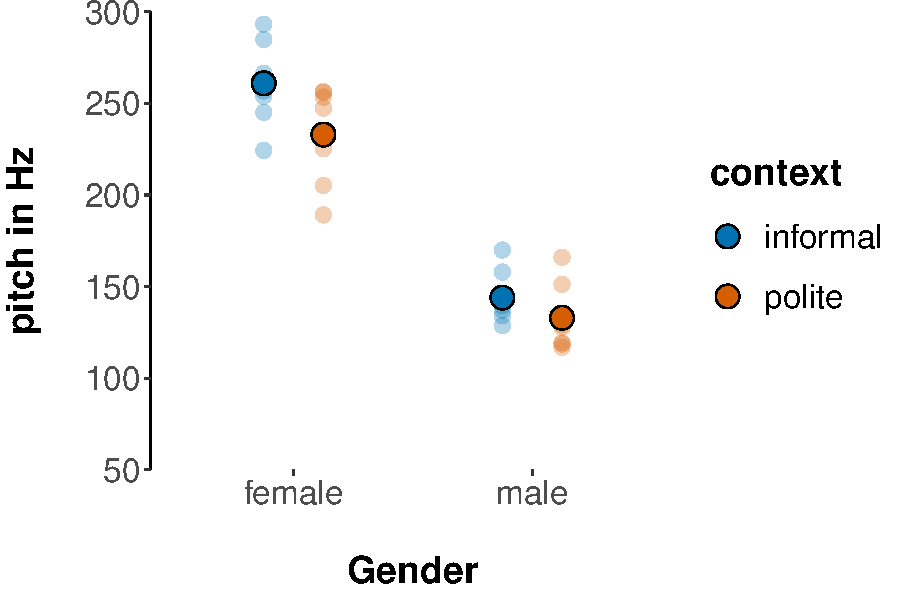
\includegraphics[width = \textwidth]{pics/basic_data_plot.pdf}
    \caption{Basic plot of the data. \mf{make me pretty}}
     \label{fig:BasicPlotData_data}
\end{figure}

Another way of looking at the data in connection with our research hyptheses is in Figure~\ref{fig:BasicPlotData_table}.

\begin{figure}[h]
  \centering
    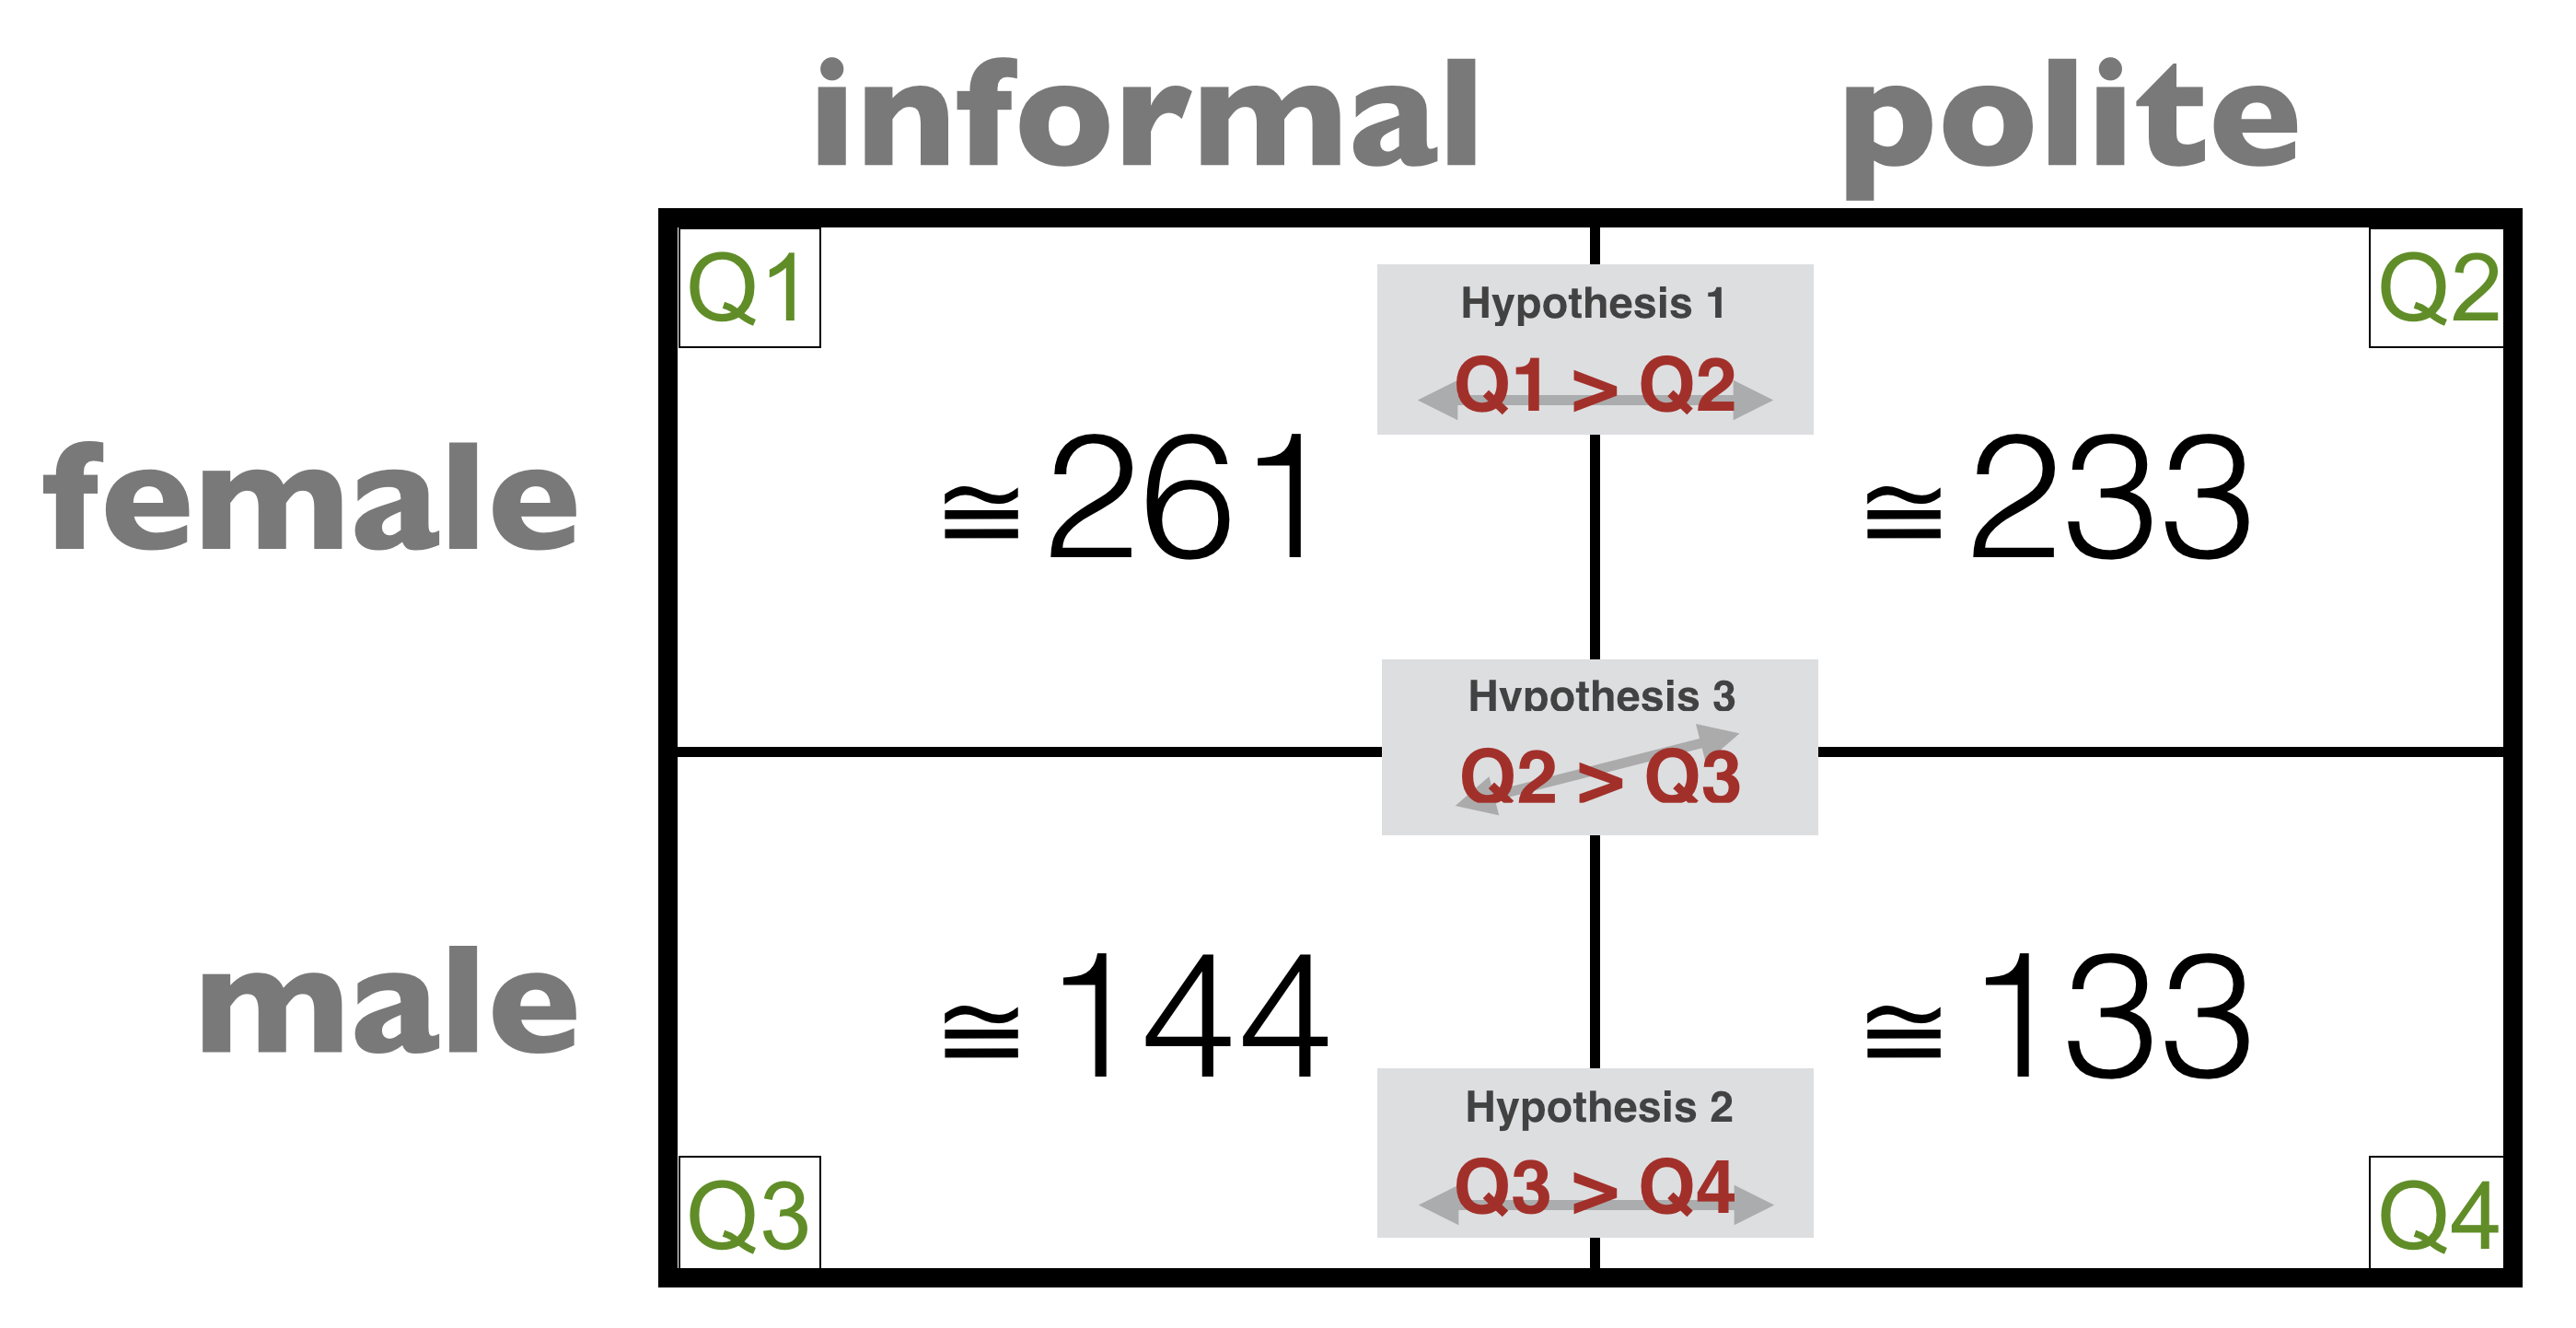
\includegraphics[width = \textwidth]{pics/table_mean_hypotheses.png}
    \caption{Means of each design cell \& research hypotheses.}
    \label{fig:BasicPlotData_table}
\end{figure}


\mf{Next steps: give the table of means; say how above comparisons translate into a comparison of cells in that table}

\newpage

\begin{InfoBox}[t]
\centering
\colorbox{mygray}{\centering
  \begin{minipage}{1.0\textwidth}

    \emph{Bayesian inference: priors, likelihoods and posteriors}
    \medskip

    Jones is a rational scientist. She has recently inherited her grandma's lucky coin. Grandma
    used this coin many times during Jones' childhood to determine whether Jones was allowed a
    sweet or not. Jones suspects that grandma's coin might be a trick coin, but she is not
    sure. She is determined to find out. How? Well, naturally, by rationally updating her
    \emph{prior beliefs} about the coin's bias to obtain a new \emph{posterior belief} based on
    emprical observation (outcomes of coin flips). Central to this updating is Jones'
    \emph{likelihood function}, which encodes how likely each relevant coin bias may have
    generated the observed data. --- Sounds fancifully abstract? But is fairly intuitive.
    Consider this example.
    
    \paragraph{Prior beliefs.} Jones initially believes that the coin is either biased towards
    heads or biased towards tails, and that both of these possibilities are equally likely. She
    also believes that, if biased towards heads, the coin is three times more likely to come up
    heads; and equally but in reverse for a bias towards tails. Numerically, Jones' \emph{prior
      beliefs} can  be written as, where $\theta \in [0;1]$ is the coin's bias: $P(\theta = 0.5)
    = \nicefrac{1}{2}$, $P(\theta = \nicefrac{3}{4}) = \nicefrac{2}{6}$, and $P(\theta =
    \nicefrac{1}{4}) = \nicefrac{1}{6}$.

    \paragraph{Likelihood.} The bias $\theta$ is, by definition, the probability of the coin
    landing heads on the next trial. Let's assume that Jones tosses the coin only once (hm,
    maybe not so rational a scientist after all? or just too busy?). Let $D$ be the set of
    potential outcomes of this experiment, namely $D = \set{\text{heads}, \text{tails}}$. The
    \emph{likelihood function} determines the likelihood of observing each datum $d \in D$ for
    each $\theta$, which in our case is just rather trivial: $P(D = \text{heads} \mid \theta) =
    \theta$ and $P(D = \text{tails} \mid \theta) = 1 - \theta$.

    \paragraph{Posterior beliefs.} Jones observes that the coin landed heads. What should she
    believe now. By \emph{Bayes rule} her posterior beliefs are defined like so:
    \begin{align*}
      P(\theta \mid D = \text{heads}) = \frac{P(\theta) P(D = \text{heads} \mid \theta)}{\sum_{\theta'}P(\theta') P(D = \text{heads} \mid \theta')}
    \end{align*}
    




  \end{minipage} \par
  } \par
  \begin{center}
    Info Box 1: Priors, likelihood and posteriors in Bayesian inference.
  \end{center}
  % \caption{\label{InfoBox:asymptotic_CIs} Here is my caption}  
\end{InfoBox}






\printbibliography[heading=bibintoc]

\end{document}
